\documentclass[12pt]{article}

% Language setting
\usepackage[utf8]{inputenc}
\usepackage[bulgarian]{babel}

% --------------------- Packages  --------------------
% Use biblatex
\usepackage{biblatex}
\addbibresource{bibliography.bib}
% Table thickness
\usepackage{ctable}
% Equations: SI units
\usepackage{siunitx}
% Approximately equal
\usepackage{amssymb}
% degrees symbol
\usepackage{gensymb}
% warning box
\usepackage{pifont,mdframed}

\newenvironment{warning}
  {\par\begin{mdframed}[linewidth=2pt, linecolor=white]%
    \begin{list}{}{\leftmargin=1cm
                   \labelwidth=\leftmargin}\item[\Large\ding{43}]}
  {\end{list}\end{mdframed}\par}

% --------------------- Title  --------------------
\addbibresource{bibliography.bib}

\begin{document}

% Anfang der Titelseite________________________________________________________________________________
\begin{titlepage}
	\flushleft
% 	\begin{center}
	%{\scshape\Large Werkstoffe III \hspace{2.5cm} Laborbericht \hspace{2.5cm}HS 2022 \par}
	{\scshape\Large Протокол IX \hspace{2cm} Механика - практикум\par}
	\vspace{5cm}
	{\huge\bfseries Уред на Обербек\par}
	\vspace{1cm}
	{\LARGE\bfseries Лабораторно упражнение №6\par}
	\vspace{5cm}
    % {\LARGE\bfseries Физически Факлутет към Софийски Университет ``Св. Климент Охридски \par}
    {\LARGE\bfseries Виолета Кабаджова, \par}
%   {\LARGE\bfseries Group: X\par}
    {\large\bfseries ККТФ, фак. номер: 3PH0600026\par}
	\vspace{1cm}
	
	{\large Физически Факултет, 
	
	Софийски Университет "Св. Климент Охридски"
	
	15 ноември 2022 г.\par}
	
\end{titlepage}

\section{Теоритична част}\label{sec:theoretical-part}
\begin{figure}
    \centering
    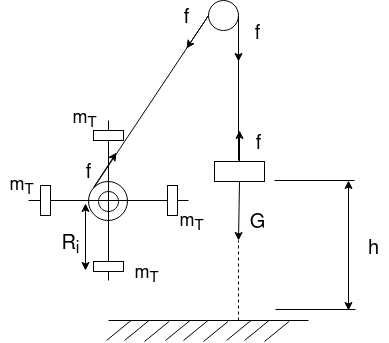
\includegraphics[width=0.5\textwidth]{images/oberbeck.drawio.png}
    \caption{Схема на уред на Обербек}
    \label{fig:setup}
\end{figure}

На фиг. \ref{fig:setup} е илюстриран т.нар. уред на Обербек. Към ос под прав ъгъл неподвижно са закрепени четири пръчки с радиус $R_i$, на всяка от които има възможност да се слага допълнителна тежест. Към оста са закрепени две шайби с различен радиус r, посредством които чрез нишка дотук описаната част се закрепя към макара. От другата страна на тази макара се поставят различни тежести $m_i$. Между най-горно и най-долно положение на масата $m_i$ има поставени фотоклетки на разстояние h една от друга. При пускане на масата $m_i$ от горното ѝ положение под действие на силата на тежестта си, тя започва да се движи равноускорително и като следствие приборът на Обербек се движи по същия начин. Пренебрегваме силите на триене, масата на макарата и приеме, че нишката е безтегловна, неразтеглива и неприплъзваща се под действие на момента на силите на опън $\vec{f}$. Телата с маса $m_i$ ще се движат праволинейно и равноускорително по закона $m_ia = m_ig - f$, откъдето следва, че:

\begin{equation}\label{eq:f}
f = m_i(g-a)    
\end{equation}

Посредством уреда на Обербек можем да изследваме законите за въртеливите движения, а именно основното ураввнение на въртеливо движение на твърдо тяло около неподвижна ос: уравнение \ref{eq:main-rotation}, където $M_z$ е моментът на приложената сила ($[M] = N.m$), $I$ - инерчният момент на въртящото тяло ($[I] = kg.m^2$), $\beta_z$ - ъгловото ускорение на тялото, ($[\beta_z] = s^{-2}$).

Тъй като инерчният момент на едно тяло спрямо дадена ос на въртене е постоянна величина, валидността на основното уравнение можем да проверим посредством доказване на равнество \ref{eq:i-const} за n измервания на $M_z$ и $\beta_z$ в различни ситуации. 

\begin{equation}\label{eq:main-rotation}
    M_z = I \beta_z
\end{equation}

\begin{equation}\label{eq:i-const}
    \frac{M_z}{\beta_z} = I = const.
\end{equation}

От уравнение \ref{eq:f} следва уравнение \ref{eq:M-z} за моментът на силата $f$, който действа на уреда на Обербек спрямо неговата ос на въртене. В него $r$ е радиусът на основната шайба, а $\alpha$ е ъгълът между $\vec{r}$ и $\vec{f}$. 

\begin{equation}\label{eq:M-z}
    M_z = rfsin\alpha = rm_i(g-a)
\end{equation}

При праволинейно равнопременливо движение ускорението съвпада с тангенциалното такова, откъдето следва, че телата с маса $m_i$ за време $t_i$ изминават път $h$ по закона за равноускорително движение без начална скорост (ур. \ref{eq:a} и \ref{eq:beta-z}).

\begin{equation}\label{eq:a}
    a = \frac{2h}{t_i^2}
\end{equation}

\begin{equation}\label{eq:beta-z}
    \beta_z = \frac{a}{r} = \frac{2h}{rt_i^2}
\end{equation}

Оттук проверката на уравнение \ref{eq:i-const} се свежда до проверката на уравнение \ref{eq:work-formula}.
\begin{equation}\label{eq:work-formula}
    I = \frac{M_z}{\beta_z} = \frac{rm_i(g-a)}{\beta_z} = \frac{m_ir^2(gt_i^2 - 2h)}{2h} = const.
\end{equation}


\section{Експериментална част}

\subsection{Задача: Определяне на инерчния момент I на прибора на Обербек (без допълнителни тела) и проверка на основното уравнение на въртеливите движения}

За целта поставяме различни тежести $m_0$ до $m_4$ от страната на уреда, на която има фотоклетки. Измерванията записваме в таблици \ref{tbl:m_0} до \ref{tbl:m_4}. I пресмятаме по формула \ref{eq:work-formula} и записваме в таблица \ref{tbl:I-s}. Грешката за I пресмятаме по формула \ref{eq:i-abs-err} и виждаме, че в действителност $I = const.$ за отделните стойности в рамките на грешките им.

\begin{equation}\label{eq:i-abs-err}
    \Delta I = \pm I \left(\frac{\Delta m_i}{m_i} + 2 \frac{\Delta r}{r} + \frac{t_i^2\Delta g + 2gt_i\Delta t_i + 2\Delta h}{gt_i^2 - 2h} + \frac{\Delta h}{h}\right)
\end{equation}

\begin{table}[h]
\begin{center}
\begin{tabular}{|l|l|l|l|}\hline
N &t_i, [s] &t_i - \bar{t}, [s] &(t_i - \bar{t})^2\cdot10^{-4}, [s] \\ \hline
\specialrule{.1em}{0em}{0em}
1 &1.509 &0.002 &0.04 \\ \hline
2 &1.437 &-0.067 &49 \\ \hline
3 &1.433 &-0.074 &54.76 \\ \hline
4 &1.533 &0.026 &6.76 \\ \hline
5 &1.623 &0.116 &134.56 \\ \hline
\specialrule{.1em}{0em}{0em}
& \bar{t}_0 = 1.507 \pm 0.078 & & (\Sigma_{i=1}^5 (t - \bar{t})^2)\cdot 10^{-4} = 61.28 \\ \hline
\end{tabular}
\caption{\label{tbl:m_0}Многократно измерване на времето за изминаване на разстоянието h от най-горно до най-долно положение за маса m_0 = 53.8 g.}
\end{center}
\end{table}


\begin{table}[h]
\begin{center}
\begin{tabular}{|l|l|l|l|}\hline
N &t_i, [s] &t_i - \bar{t}, [s] &(t_i - \bar{t})^2\cdot10^{-4}, [s] \\ \hline
\specialrule{.1em}{0em}{0em}
1 &1.15 &-0.0066 &0.4356 \\ \hline
2 &1.16 &0.0034 &0.1156 \\ \hline
3 &1.145 &-0.0116 &1.3456 \\ \hline
4 &1.161 &0.0044 &0.1936 \\ \hline
5 &1.167 &0.0104 &1.0816 \\ \hline
\specialrule{.1em}{0em}{0em}
& \bar{t}_1 = 1.1566 \pm 0.0089 & & (\Sigma_{i=1}^5 (t - \bar{t})^2)\cdot 10^{-4} = 0.7930 \\ \hline
\end{tabular}
\caption{\label{tbl:m_1}Многократно измерване на времето за изминаване на разстоянието h от най-горно до най-долно положение за маса m_1 = 93.8 g.}
\end{center}
\end{table}


\begin{table}[h]
\begin{center}
\begin{tabular}{|l|l|l|l|}\hline
N &t_i, [s] &t_i - \bar{t}, [s] &(t_i - \bar{t})^2\cdot10^{-4}, [s] \\ \hline
\specialrule{.1em}{0em}{0em}
1 &1.025 &0.0514 &26.4196 \\ \hline
2 &0.961 &-0.0126 &1.5876 \\ \hline
3 &0.999 &0.0254 &6.4516 \\ \hline
4 &0.938 &-0.0356 &12.6736 \\ \hline
5 &0.945 &-0.0286 &8.1796 \\ \hline
\specialrule{.1em}{0em}{0em}
& \bar{t}_2 = 0.9736 \pm 0.0372 & & (\Sigma_{i=1}^5 (t - \bar{t})^2)\cdot 10^{-4} = 13.828 \\ \hline
\end{tabular}
\caption{\label{tbl:m_2}Многократно измерване на времето за изминаване на разстоянието h от най-горно до най-долно положение за маса m_2 = 133.8 g.}
\end{center}
\end{table}


\begin{table}[h]
\begin{center}
\begin{tabular}{|l|l|l|l|}\hline
N &t_i, [s] &t_i - \bar{t}, [s] &(t_i - \bar{t})^2\cdot10^{-4}, [s] \\ \hline
\specialrule{.1em}{0em}{0em}
1 &0.876 &0.0218 &4.7524 \\ \hline
2 &0.845 &-0.0092 &0.8464 \\ \hline
3 &0.834 &-0.0202 &4.0804 \\ \hline
4 &0.847 &-0.0072 &0.5184 \\ \hline
5 &0.869 &0.0148 &2.1904 \\ \hline
\specialrule{.1em}{0em}{0em}
& \bar{t}_3 = 0.8542 \pm 0.0176 & & (\Sigma_{i=1}^5 (t - \bar{t})^2)\cdot 10^{-4} = 3.097 \\ \hline
\end{tabular}
\caption{\label{tbl:m_3}Многократно измерване на времето за изминаване на разстоянието h от най-горно до най-долно положение за маса m_3 = 173.8 g.}
\end{center}
\end{table}


\begin{table}[h]
\begin{center}
\begin{tabular}{|l|l|l|l|}\hline
N &t_i, [s] &t_i - \bar{t}, [s] &(t_i - \bar{t})^2\cdot10^{-4}, [s] \\ \hline
\specialrule{.1em}{0em}{0em}
1 &0.757 &0.0052 &0.2704 \\ \hline
2 &0.741 &-0.0108 &1.1664 \\ \hline
3 &0.772 &0.0202 &4.0804 \\ \hline
4 &0.756 &0.0042 &0.1764 \\ \hline
5 &0.733 &-0.0188 &3.5344 \\ \hline
\specialrule{.1em}{0em}{0em}
& \bar{t}_4 = 0.7518 \pm 0.0152 & & (\Sigma_{i=1}^5 (t - \bar{t})^2)\cdot 10^{-4} = 2.307 \\ \hline
\end{tabular}
\caption{\label{tbl:m_4}Многократно измерване на времето за изминаване на разстоянието h от най-горно до най-долно положение за маса m_4 = 213.8 g.}
\end{center}
\end{table}

\begin{table}[h]
\begin{center}
\begin{tabular}{|l|l|}\hline
m_i, [g] &I_i, [kgm^2] \\ \hline
\specialrule{.1em}{0em}{0em}
53.8 &1.6158 \pm 0.1775\\ \hline
93.8 &1.6296 \pm 0.0048\\ \hline
133.8 &1.6169 \pm 0.0046\\ \hline
173.8 &1.5858 \pm 0.0044\\ \hline
213.8 &1.4737 \pm 0.0041\\ \hline
\end{tabular}
\caption{\label{tbl:I-s} Изчислените инерчни моменти $I_i$ за всяка от масите с техните грешки.}
\end{center}
\end{table}


\subsection{Задача: Определяне на инерчния момент на допълнителните тела в зависимост от растоянието им $R_i$ до оста на въртене}

При фиксирано разстояние $h$ и маса $m = 213.8g$ измерваме многократно времето на преминаване на тялото между двете фотоклетки при различни разстояния $R_i$ от оста на въртене до центъра на масите на допълнителните тела. В таблица \ref{tbl:task-2-I-s} записваме средните стойности на времето $t_i$, за което тялото преминава разстоянието h между фотоклетките при сложени допулнителни тежести върху уреда на Обербек на разстояние $R_i$. В таблицата записваме изчисления по формула \ref{eq:work-formula} инерчен момент $I_{ci}$ на съответната система, както и изчисления инерчен момент на всяко от допълнителните тела с маса $m_T$ (виж фиг. \ref{fig:setup}) по формулата $I_c = I_o + 4I_{Ri}$, където $I_o$ е средната стойност на получения в предишната задача инерчен момент на уреда на Обербек.

На фиг. \ref{fig:data} е представена зависимостта $I_R(R^2)$. Ако допълнителните тела могат да се разглеждат като материални точки ($I_R = m_T R^2$), графиката на тази зависимост би трябвало да бъде права линия, минаваща орез началото на координатната система. При R \rightarrow $R_{min}$ размерите на телата вече не могат да се пренебрегват, поради което зависимостта няма да клони към нула при R, клонящо към 0. Оттук все пак можем да заключим, че съгласно графиката на фиг. \ref{fig:data} до съответния радиус, при който са направени измерванията допълнителните тежести могат да се считат за материални точки.

\begin{table}[h]
\begin{center}
\begin{tabular}{|l|l|l|l|l|}\hline
N &R_i, [cm] &t_i, [s] &I_{ci}, [kgm^2] &I_{Ri}, [kgm^2] \\\hline
\specialrule{.1em}{0em}{0em}
0 &24.5 &2.3668 &16.0816 &3.6243 \pm 0.0055\\\hline
1 &21.5 &2.1784 &13.5979 &3.0034 \pm 0.0249 \\\hline
2 &18.5 &1.9256 &10.5888 &2.2511 \pm 0.0436\\\hline
3 &15.5 &1.7178 &8.3930 &1.7022 \pm 0.0103\\\hline
4 &12.5 &1.4008 &5.5257 &0.9853 \pm 0.0086\\\hline
5 &9.5 &1.20768 &4.0646 &0.6201 \pm 0.0191\\\hline
6 &6.5 &1.0132 &2.8119 &0.3069 \pm 0.0340\\\hline
\end{tabular}
\caption{\label{tbl:task-2-I-s} Изчислените инерчни моменти $I_{Ri}$ за всеки от радиусите с техните грешки.}
\end{center}
\end{table}

\begin{figure}
    \centering
    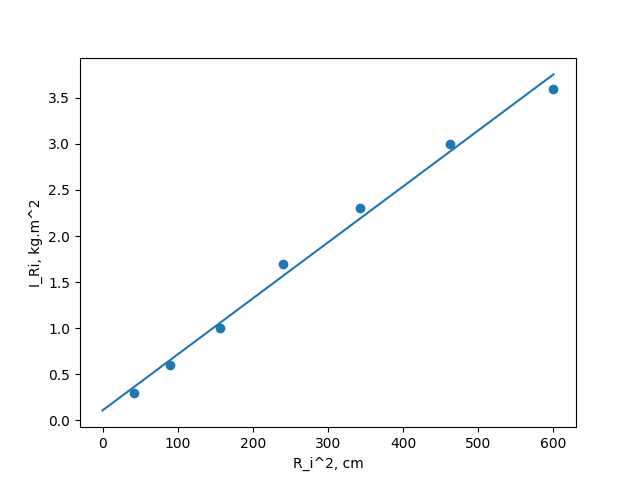
\includegraphics[width=0.6\textwidth]{images/data.png}
    \caption{Зависимостта I_R(R^2)}
    \label{fig:data}
\end{figure}

\end{document}
